\subsection{Zarządzanie użytkownikami}

W ramach pracy zaimplementowano prosty system zarządzania użytkownikami. System
pozwala tworzyć i usuwać konta użytkowników.

Tworzenie kont powinno być wykonywane przez administratora. Użytkownicy mogą
jedynie zmieniać hasło do swojego konta i korzystać z udostępnionych im punktów
końcowych. W celu ułatwienia pracy administratorom, aplikacja pozwala na
tworzenie dowolnej ilości kont za pomocą jednej operacji. Administrator podaje
nazwę konta, która zawiera ciąg znaków ``\verb|{}|'', grupę użytkowników, do
której będą należały konta oraz pożądaną ilość nowych kont. Interfejs tworzenia
użytkowników został przedstawiony na rysunku \ref{userCreationFigure}.

\begin{figure}[h]
    \centering
    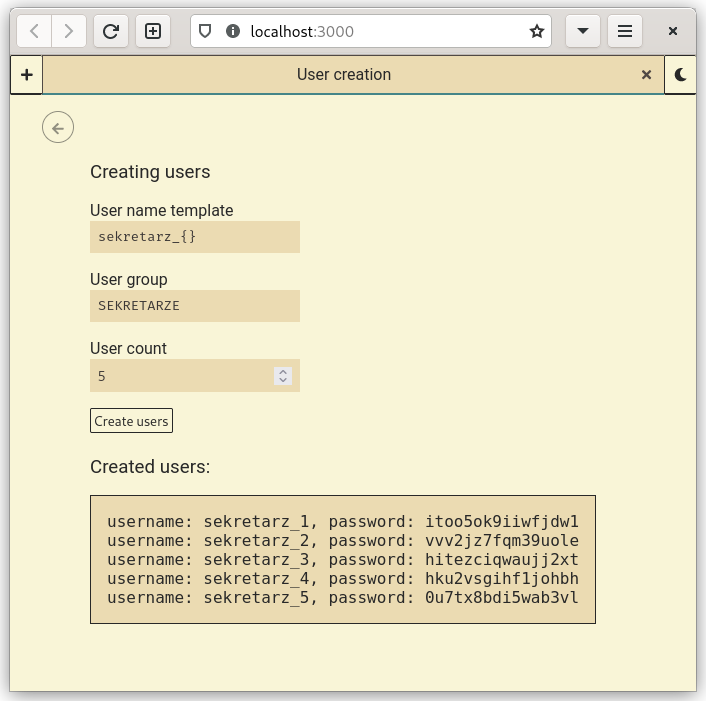
\includegraphics[width=.7\textwidth]{./img/creating_users.png}
    \caption{Interfejs tworzenia użytkowników}
    \label{userCreationFigure}
\end{figure}

Ciąg znaków ``\verb|{}|'' zostanie zastąpiony numerem. Program zacznie od numeru
``1'' i sprawdzi, czy w bazie danych znajduje się już użytkownik o takiej
nazwie. Jeśli nazwa użytkownika już istnieje, zwiększy numer o jeden i spróbuje
ponownie. Jeśli nazwa użytkownika jest wolna, stworzy nowe konto. Program będzie
powtarzał czynność, dopóki nie utworzy pożądanej ilości kont użytkowników.

Wygenerowane hasła są przechowywane jedynie w pamięci RAM podczas generowania
kont użytkownika. W bazie danych zapisywane są hasła mieszane za pomocą
algorytmu Argon2. Tak przetworzone hasła nie mogą zostać użyte do zalogowania
się do systemu. Po odesłaniu haseł do administratora w odpowiedzi HTTP,
oryginalna postać haseł przestaje istnieć w systemie.

Zarządzanie stworzonymi użytkownikami jest ograniczone do możliwości usuwania
kont użytkowników z systemu. Interfejs zarządzania użytkownikami został
przedstawiony na rysunku \ref{userManagementFigure}.

\begin{figure}[h]
    \centering
    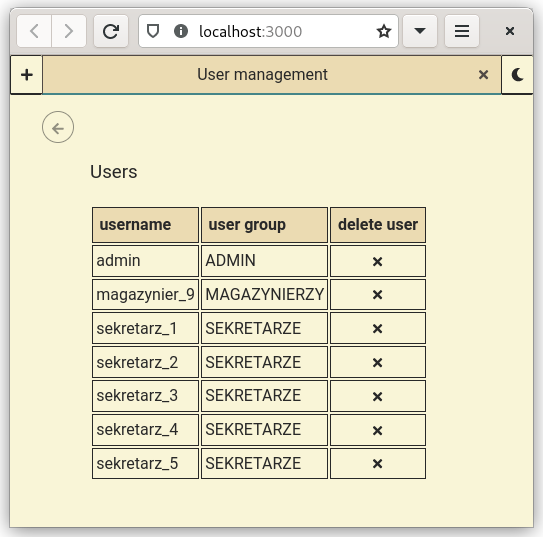
\includegraphics[width=.6\textwidth]{./img/user_management.png}
    \caption{Interfejs zarządzania kontami użytkowników}
    \label{userManagementFigure}
\end{figure}
